\chapter{Software Tools}\label{ch:tools}

\section{AstroTaverna Plugin}
\hrefnote{http://www.taverna.org.uk/}{Taverna}~\citep{Wolstencroft2013} is an open source, domain-independent scientific workflow management system that has grown popular in fields like bioinformatics, chemistry, text mining, and image analysis. It is a suite of tools including Taverna Workbench, a desktop client application used to graphically design, create, edit and execute scientific workflows. Taverna workflows can also be executed on the command line or on an installation of the Taverna Server.

\begin{figure}[h!]
\begin{center}

  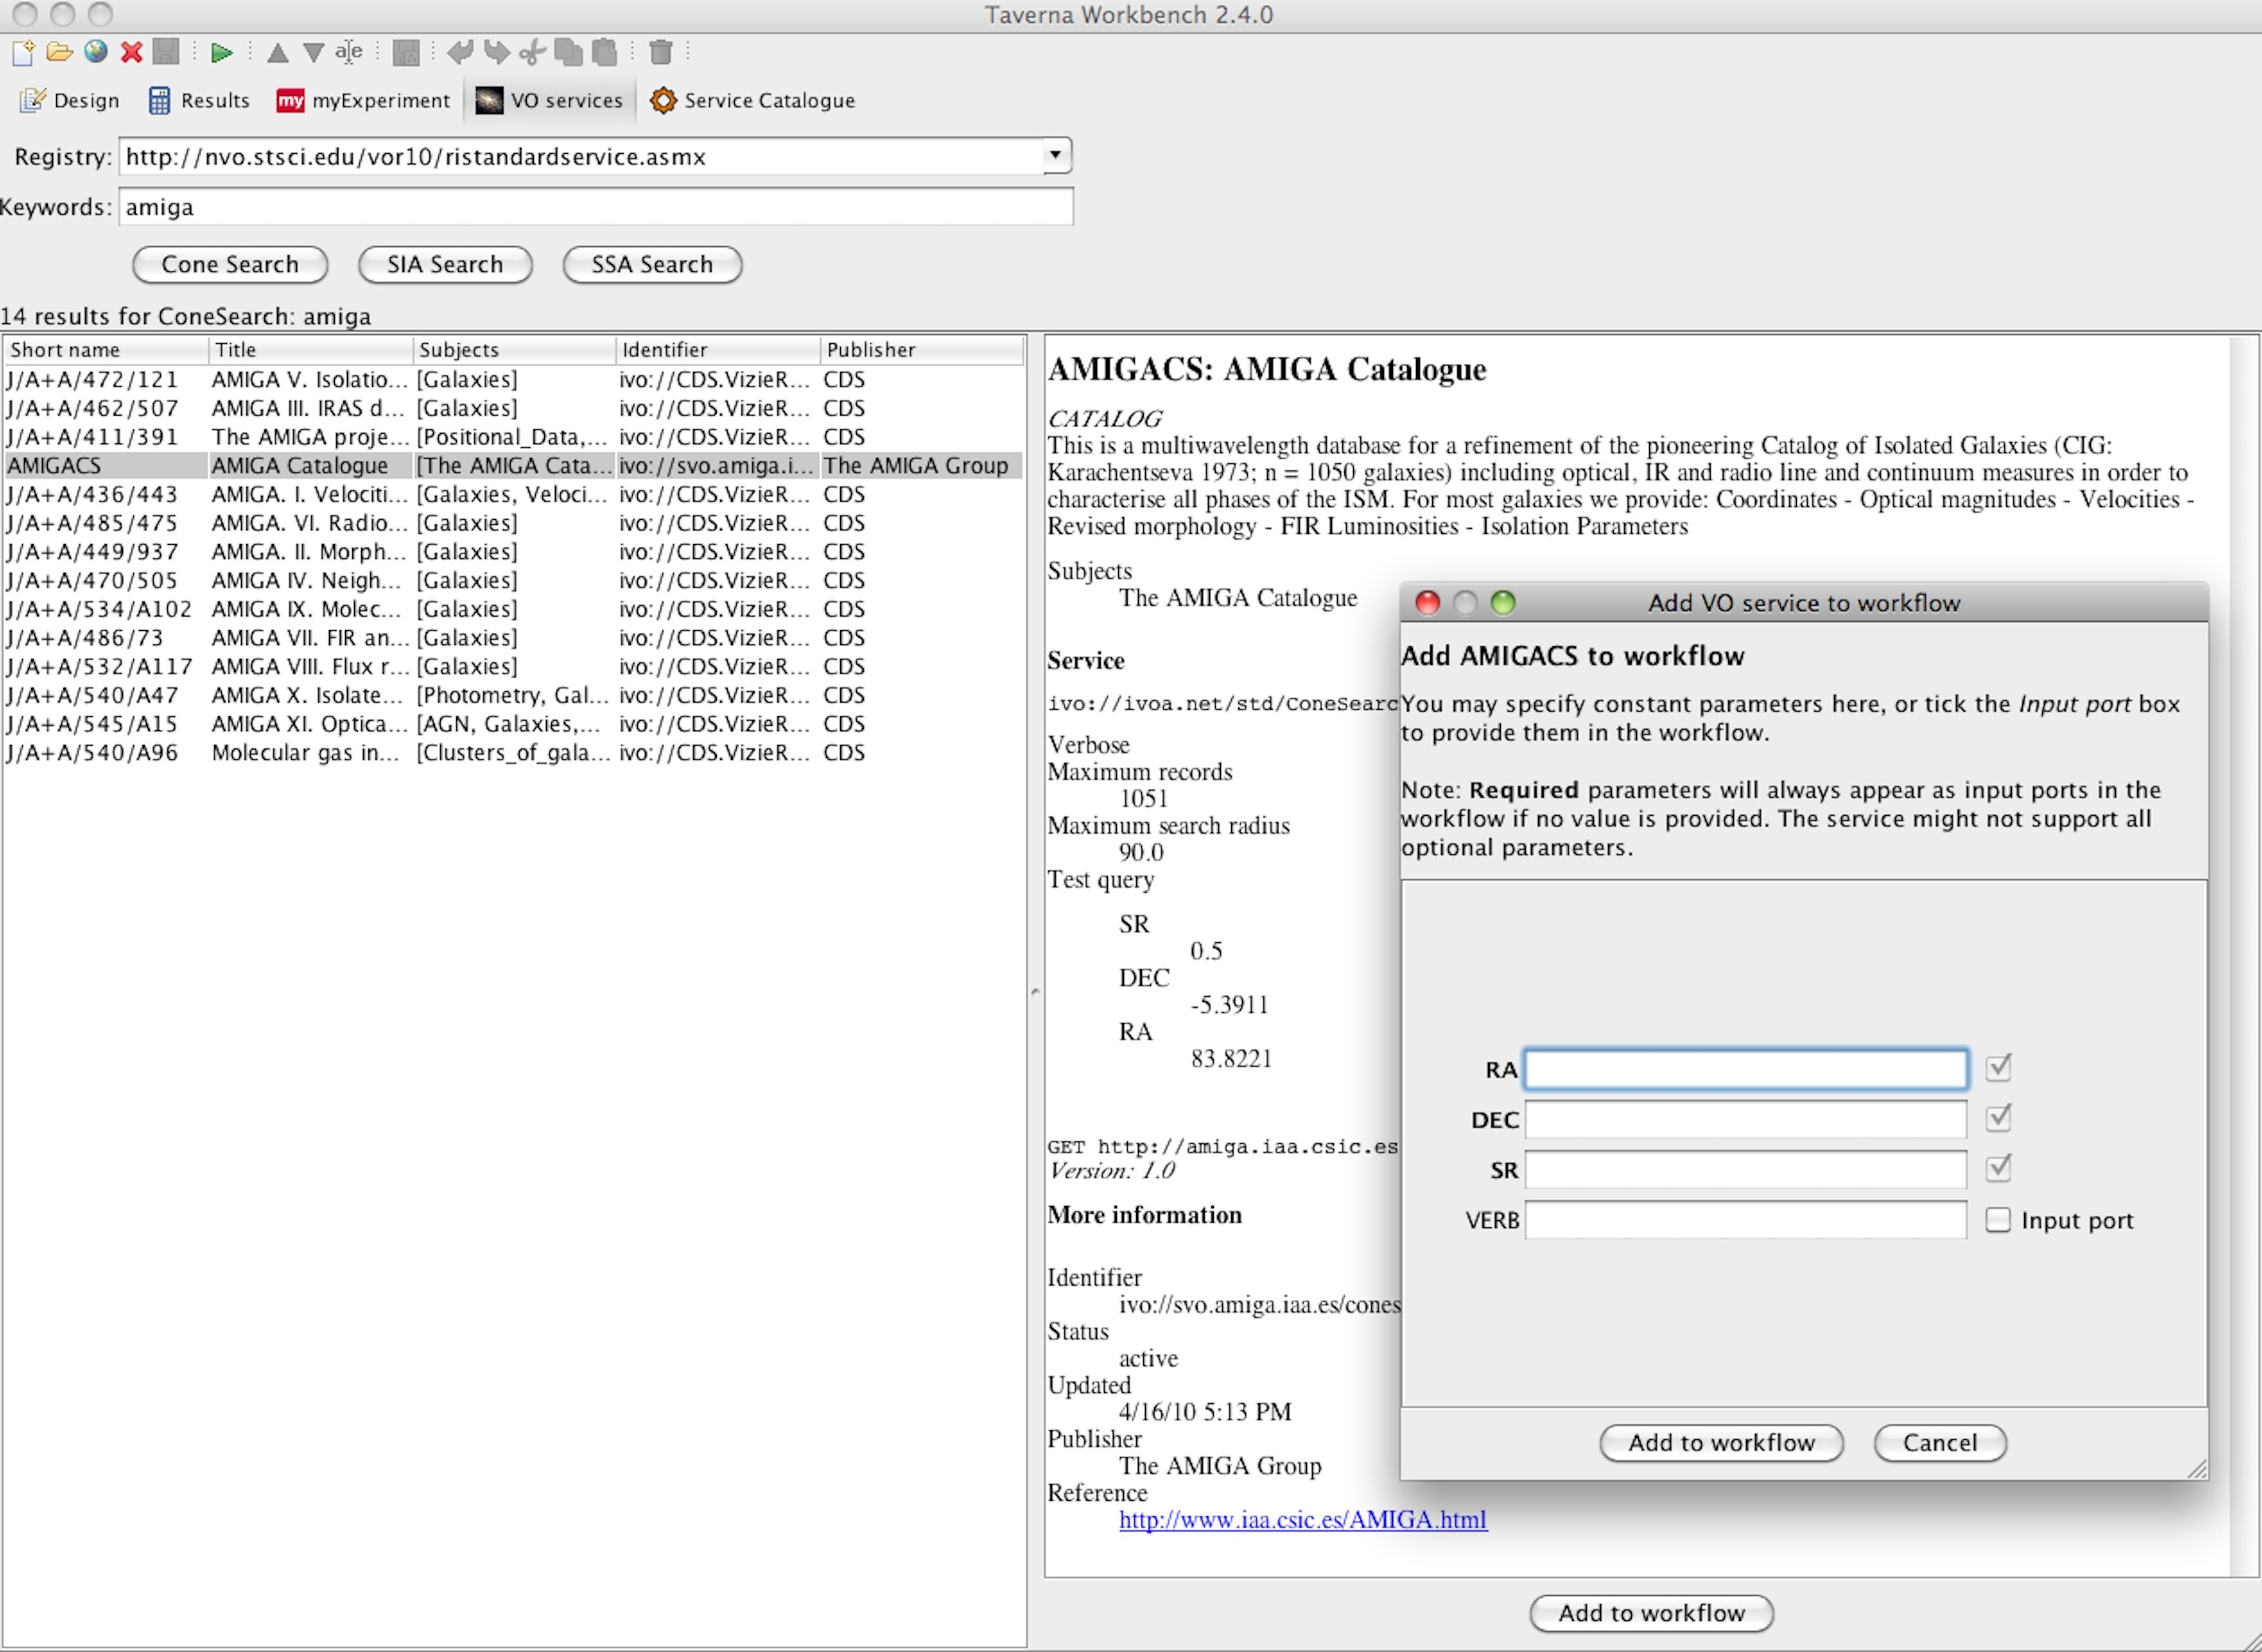
\includegraphics{gfx/VODiscovery.jpg}
  \caption{VO Discovery in AstroTaverna Plugin}
  \label{fig:vodiscovery}
\end{center}
\end{figure}

Figure \ref{fig:vodiscovery} shows the discovery functions of AstroTaverna plugin.

\section{AMIGA IPython Notebook Server}

Lorem ipsum dolor sit amet,  \ac{API}  consectetur adipisicing elit, sed do eiusmod tempor incididunt ut labore et dolore magna aliqua. Ut enim ad minim veniam \ac{IVOA}, quis nostrud exercitation ullamco laboris nisi ut aliquip ex ea commodo consequat. Duis aute irure dolor in reprehenderit in voluptate velit  \ac{UML}  esse cillum dolore eu fugiat nulla pariatur \ac{VO}. Excepteur sint occaecat cupidatat non proident, sunt in culpa qui officia deserunt mollit anim id est laborum. 


Aenean bibendum dui in sem luctus dapibus. Duis eleifend ipsum quis justo tincidunt sagittis. Nullam id porttitor orci. Vestibulum ornare eu ligula vitae ultrices. Nam sit amet posuere nisl. Sed tincidunt mauris ac lectus imperdiet fermentum. Sed sodales pellentesque volutpat. Aliquam ultricies sed nisi in mollis. Maecenas ut justo et felis dictum feugiat. Integer vitae velit volutpat, tincidunt orci vel, facilisis libero. Interdum et malesuada fames ac ante ipsum primis in faucibus. Phasellus vel consequat ante. Morbi quis neque et justo egestas porta quis consectetur mauris. Sed venenatis sapien in elementum vestibulum. Curabitur hendrerit facilisis magna nec tincidunt. Cras id lorem elit.
